%Spelling checked 2004-04-06
C.T. Lawrence Butler has lived an alternative lifestyle since he left college at the end of the Vietnam War. With a group of actors in Boston, MA, he founded a theater production company and produced several off-off-Broadway plays including \emph{Dracula}, \emph{Sylvia Plath}, and \emph{The Marlowe Show} in Boston and \emph{Fits, Seizures and Small Complaints} in New York City. He is a self-taught cook and has held a position as a head chef in a French restaurant. He has been a vegetarian for over 30 years and written a vegetarian cookbook. He is a founding member of a worldwide, nonviolent, grassroots activist movement known as Food Not Bombs. His nonviolent direct actions against war, poverty and injustice have led to his being beaten, tortured and arrested over 50 times in the United States without ever having committed or been convicted of a crime. He is a proud father and parent to several children. He has participated in a surrogate birth and helped raise a ``step'' daughter who is a full-blooded Native American Aymara Indian from Bolivia. He has written three books: \emph{On Conflict and Consensus}, \emph{Food Not Bombs: How to Feed the Hungry and Build Community}, and, the soon to be published, \emph{Consensus for Cities of 100,000}. He travels extensively teaching and lecturing on nonviolent conflict resolution, consensus decisionmaking and grassroots political organizing. 

Before C.T. wrote \emph{On Conflict and Consensus}, and before mediation was big business, C.T. was already developing his approach to nonviolence, aka alternative conflict resolution. He had a private practice helping couples, individuals and groups mediate their conflicts. Throughout the 1980s, he was in demand for mediation and nonviolence trainings by various organizations and grassroots activist groups. During the early years of the AIDS epidemic, C.T. was recruited by the organization ACT UP Maine to teach nonviolence trainings in preparation for nonviolent direct actions related to AIDS.

\emph{On Conflict and Consensus} was published in 1987. In it, he defines his model of consensus called Formal Consensus. In the early 1990s, C.T. shifted his efforts from grassroots activism to focus his attention on teaching workshops on Formal Consensus. Since then, he has facilitated over 60 Formal Consensus workshops in the US. In addition, various organizations have sponsored workshops by C.T. in Stockholm, Ottawa, London, and Paris. A wide variety of community groups and organizations have adopted Formal Consensus as their decisionmaking process. The list includes:

\squishitemize%\begin{itemize}

	\item Co-Housing Communities

	\item Eco Villages

	\item Homeless Advocacy Organizations

	\item Native American Indian Tribes

	\item Government Agencies

	\item Boards of Directors of Non-profit Organizations

	\item Social Change Groups

	\item African Nonviolent Revolutionaries

	\item Churches

	\item Professional Organizations

	\item Covens

	\item Food Coops

	\item Alternative Schools and Colleges

	\item Anarchist Networks in Eastern Europe

	\item Artist Collectives

	\item Dance Communities

	\item Independent Media Collectives

	\item Families
\squishend%\end{itemize}


In August 1999, C.T. sustained a serious head injury. He stopped traveling and took an extended leave of absence from teaching. He reentered the field in September 2005 by teaching a 2-day workshop with the Humanities Department faculty at the University of Puerto Rico in Mayagüez. In March 2006, he presented his first ever 4-day Training for Teachers (T4T) workshop. The workshop, held in Tucson, AZ, was a tremendous success with 30 participants from across the US, including two activists from Africa. 

Currently, he is motivated to enlarge the scope of Formal Consensus by addressing the use of consensus in large organizations and the use of consensus as a form of government. His new book, \emph{Consensus for Cities of 100,000}, will address these topics and more. 


\begin{figure}[h]
\begin{center}
\fbox{
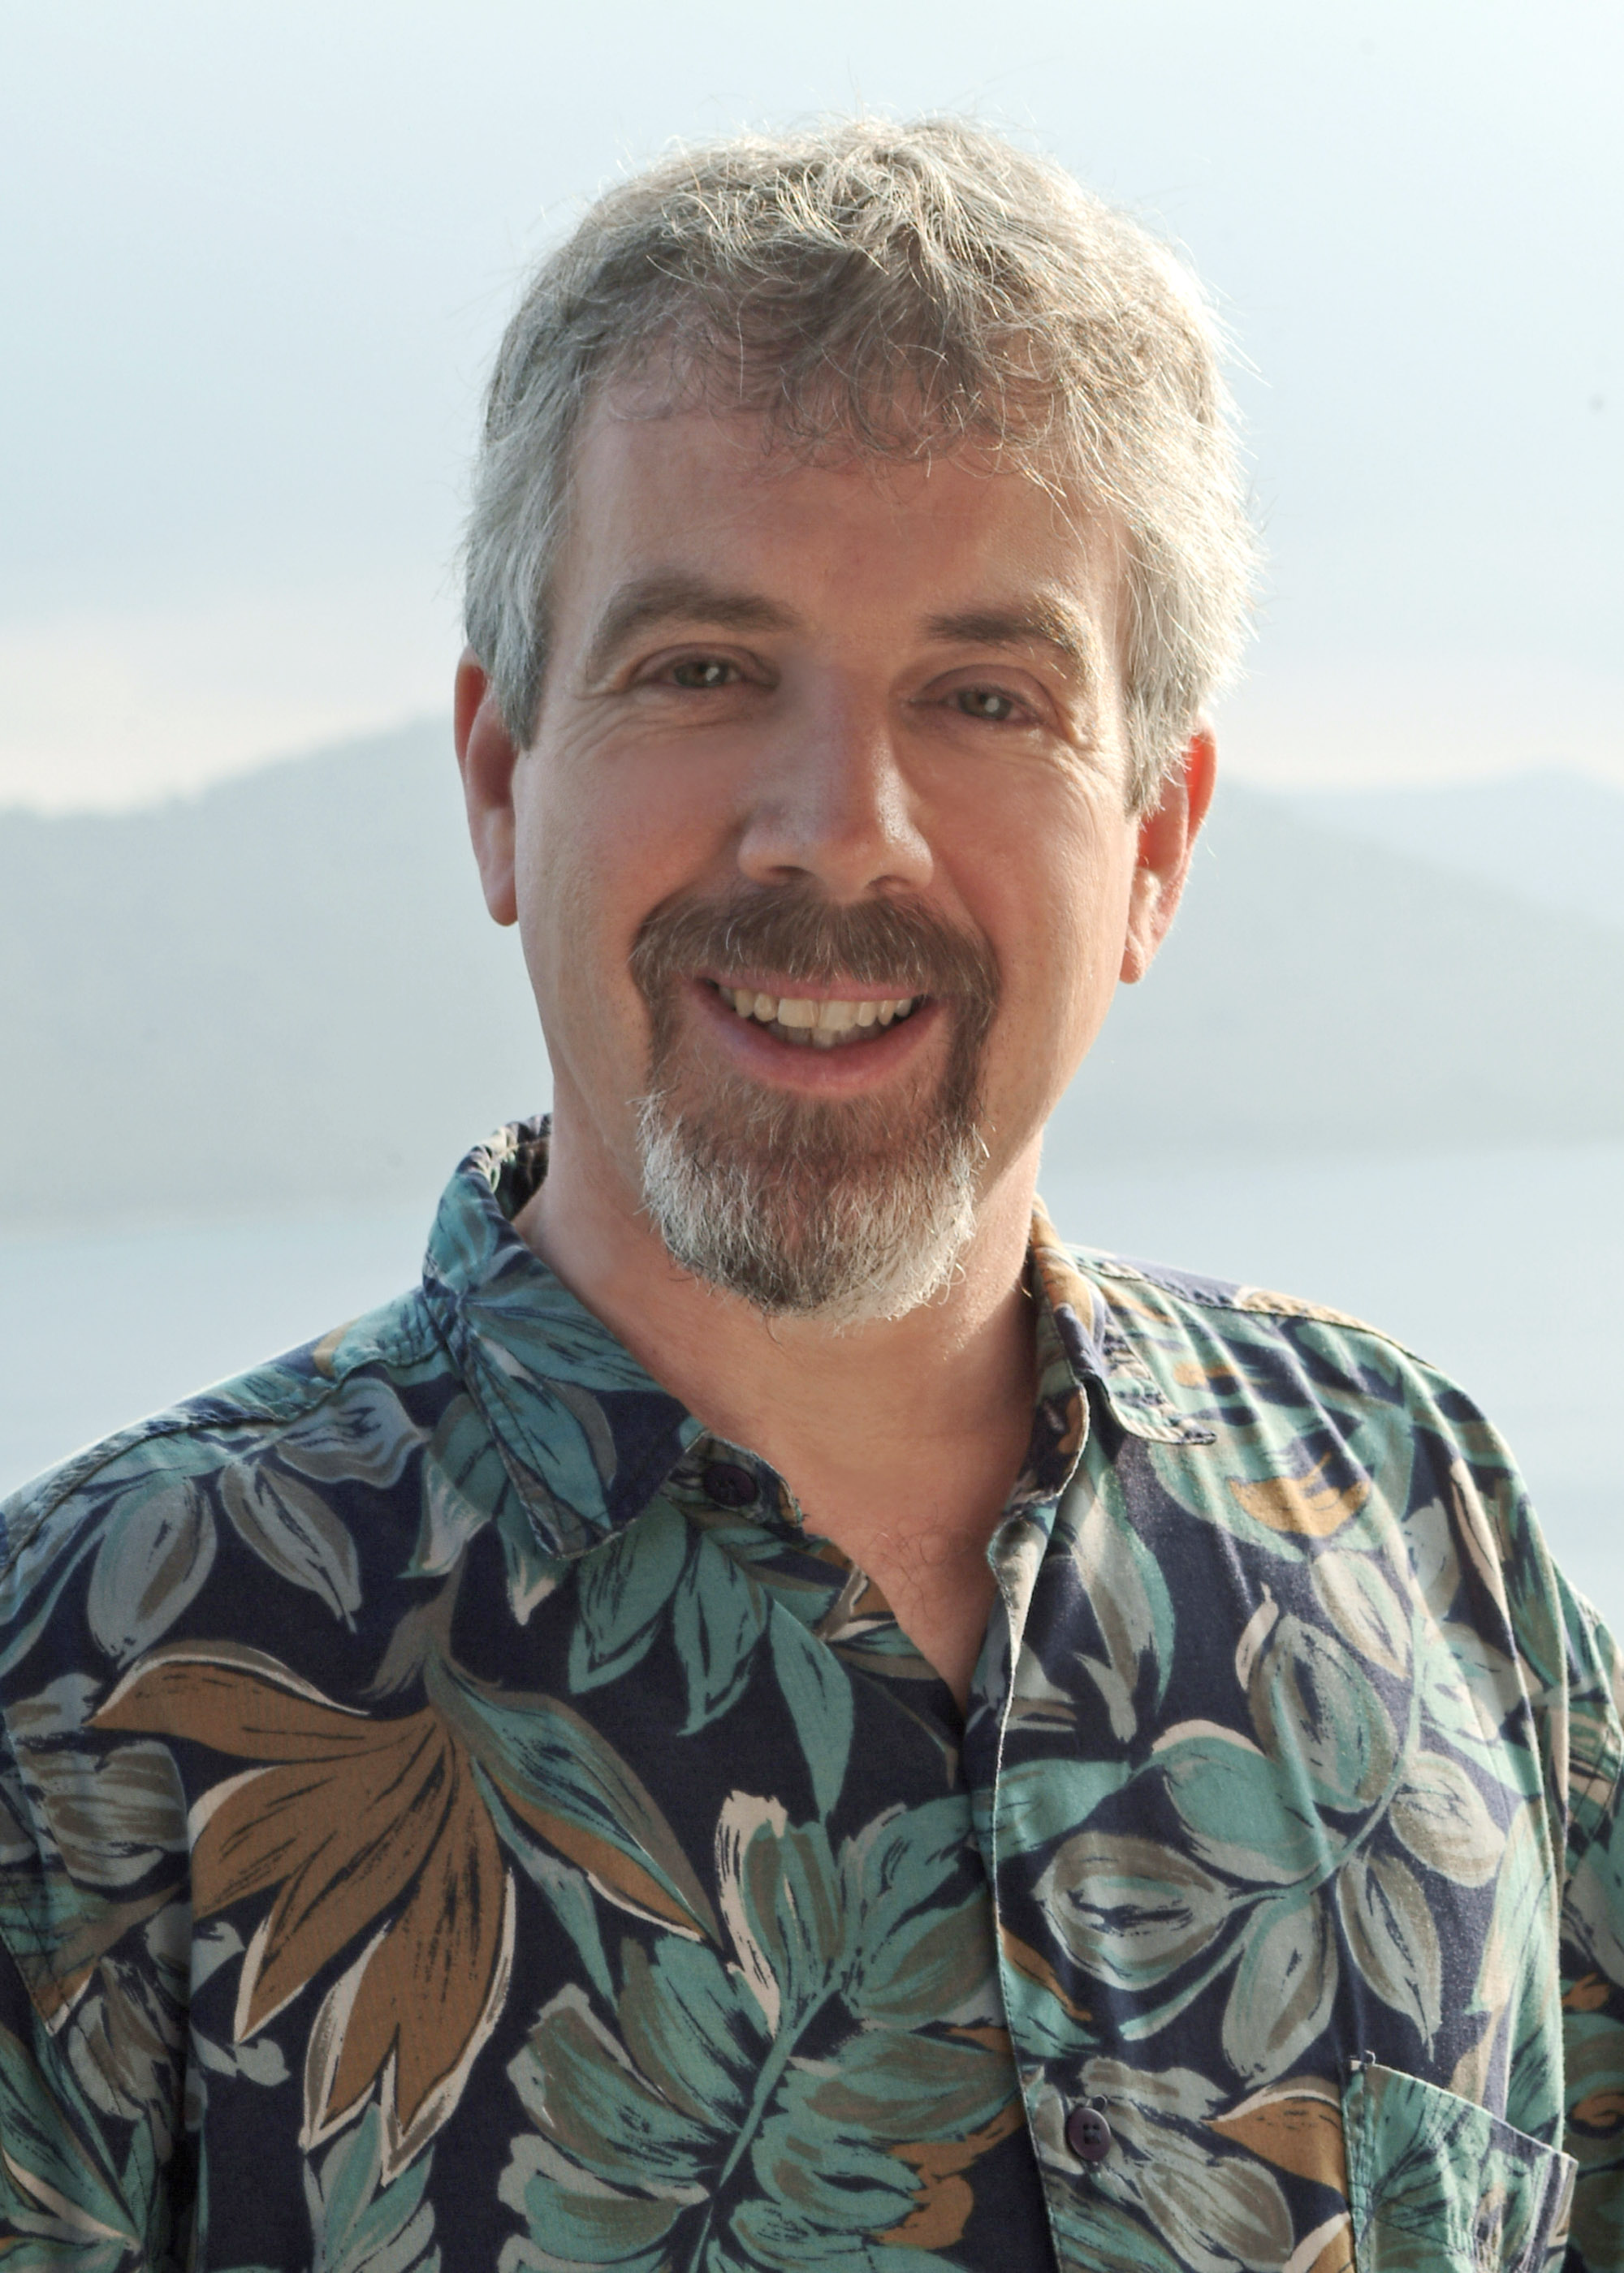
\includegraphics[width=5em]{ct05caribbean}}  %Notice how this line is different
\label{fig:ctpicture}
\end{center}
\end{figure}